% Options for packages loaded elsewhere
\PassOptionsToPackage{unicode}{hyperref}
\PassOptionsToPackage{hyphens}{url}
%
\documentclass[
]{article}
\usepackage{amsmath,amssymb}
\usepackage{iftex}
\ifPDFTeX
  \usepackage[T1]{fontenc}
  \usepackage[utf8]{inputenc}
  \usepackage{textcomp} % provide euro and other symbols
\else % if luatex or xetex
  \usepackage{unicode-math} % this also loads fontspec
  \defaultfontfeatures{Scale=MatchLowercase}
  \defaultfontfeatures[\rmfamily]{Ligatures=TeX,Scale=1}
\fi
\usepackage{lmodern}
\ifPDFTeX\else
  % xetex/luatex font selection
\fi
% Use upquote if available, for straight quotes in verbatim environments
\IfFileExists{upquote.sty}{\usepackage{upquote}}{}
\IfFileExists{microtype.sty}{% use microtype if available
  \usepackage[]{microtype}
  \UseMicrotypeSet[protrusion]{basicmath} % disable protrusion for tt fonts
}{}
\makeatletter
\@ifundefined{KOMAClassName}{% if non-KOMA class
  \IfFileExists{parskip.sty}{%
    \usepackage{parskip}
  }{% else
    \setlength{\parindent}{0pt}
    \setlength{\parskip}{6pt plus 2pt minus 1pt}}
}{% if KOMA class
  \KOMAoptions{parskip=half}}
\makeatother
\usepackage{xcolor}
\usepackage[margin=1in]{geometry}
\usepackage{color}
\usepackage{fancyvrb}
\newcommand{\VerbBar}{|}
\newcommand{\VERB}{\Verb[commandchars=\\\{\}]}
\DefineVerbatimEnvironment{Highlighting}{Verbatim}{commandchars=\\\{\}}
% Add ',fontsize=\small' for more characters per line
\usepackage{framed}
\definecolor{shadecolor}{RGB}{248,248,248}
\newenvironment{Shaded}{\begin{snugshade}}{\end{snugshade}}
\newcommand{\AlertTok}[1]{\textcolor[rgb]{0.94,0.16,0.16}{#1}}
\newcommand{\AnnotationTok}[1]{\textcolor[rgb]{0.56,0.35,0.01}{\textbf{\textit{#1}}}}
\newcommand{\AttributeTok}[1]{\textcolor[rgb]{0.13,0.29,0.53}{#1}}
\newcommand{\BaseNTok}[1]{\textcolor[rgb]{0.00,0.00,0.81}{#1}}
\newcommand{\BuiltInTok}[1]{#1}
\newcommand{\CharTok}[1]{\textcolor[rgb]{0.31,0.60,0.02}{#1}}
\newcommand{\CommentTok}[1]{\textcolor[rgb]{0.56,0.35,0.01}{\textit{#1}}}
\newcommand{\CommentVarTok}[1]{\textcolor[rgb]{0.56,0.35,0.01}{\textbf{\textit{#1}}}}
\newcommand{\ConstantTok}[1]{\textcolor[rgb]{0.56,0.35,0.01}{#1}}
\newcommand{\ControlFlowTok}[1]{\textcolor[rgb]{0.13,0.29,0.53}{\textbf{#1}}}
\newcommand{\DataTypeTok}[1]{\textcolor[rgb]{0.13,0.29,0.53}{#1}}
\newcommand{\DecValTok}[1]{\textcolor[rgb]{0.00,0.00,0.81}{#1}}
\newcommand{\DocumentationTok}[1]{\textcolor[rgb]{0.56,0.35,0.01}{\textbf{\textit{#1}}}}
\newcommand{\ErrorTok}[1]{\textcolor[rgb]{0.64,0.00,0.00}{\textbf{#1}}}
\newcommand{\ExtensionTok}[1]{#1}
\newcommand{\FloatTok}[1]{\textcolor[rgb]{0.00,0.00,0.81}{#1}}
\newcommand{\FunctionTok}[1]{\textcolor[rgb]{0.13,0.29,0.53}{\textbf{#1}}}
\newcommand{\ImportTok}[1]{#1}
\newcommand{\InformationTok}[1]{\textcolor[rgb]{0.56,0.35,0.01}{\textbf{\textit{#1}}}}
\newcommand{\KeywordTok}[1]{\textcolor[rgb]{0.13,0.29,0.53}{\textbf{#1}}}
\newcommand{\NormalTok}[1]{#1}
\newcommand{\OperatorTok}[1]{\textcolor[rgb]{0.81,0.36,0.00}{\textbf{#1}}}
\newcommand{\OtherTok}[1]{\textcolor[rgb]{0.56,0.35,0.01}{#1}}
\newcommand{\PreprocessorTok}[1]{\textcolor[rgb]{0.56,0.35,0.01}{\textit{#1}}}
\newcommand{\RegionMarkerTok}[1]{#1}
\newcommand{\SpecialCharTok}[1]{\textcolor[rgb]{0.81,0.36,0.00}{\textbf{#1}}}
\newcommand{\SpecialStringTok}[1]{\textcolor[rgb]{0.31,0.60,0.02}{#1}}
\newcommand{\StringTok}[1]{\textcolor[rgb]{0.31,0.60,0.02}{#1}}
\newcommand{\VariableTok}[1]{\textcolor[rgb]{0.00,0.00,0.00}{#1}}
\newcommand{\VerbatimStringTok}[1]{\textcolor[rgb]{0.31,0.60,0.02}{#1}}
\newcommand{\WarningTok}[1]{\textcolor[rgb]{0.56,0.35,0.01}{\textbf{\textit{#1}}}}
\usepackage{graphicx}
\makeatletter
\def\maxwidth{\ifdim\Gin@nat@width>\linewidth\linewidth\else\Gin@nat@width\fi}
\def\maxheight{\ifdim\Gin@nat@height>\textheight\textheight\else\Gin@nat@height\fi}
\makeatother
% Scale images if necessary, so that they will not overflow the page
% margins by default, and it is still possible to overwrite the defaults
% using explicit options in \includegraphics[width, height, ...]{}
\setkeys{Gin}{width=\maxwidth,height=\maxheight,keepaspectratio}
% Set default figure placement to htbp
\makeatletter
\def\fps@figure{htbp}
\makeatother
\setlength{\emergencystretch}{3em} % prevent overfull lines
\providecommand{\tightlist}{%
  \setlength{\itemsep}{0pt}\setlength{\parskip}{0pt}}
\setcounter{secnumdepth}{-\maxdimen} % remove section numbering
\newlength{\cslhangindent}
\setlength{\cslhangindent}{1.5em}
\newlength{\csllabelwidth}
\setlength{\csllabelwidth}{3em}
\newlength{\cslentryspacingunit} % times entry-spacing
\setlength{\cslentryspacingunit}{\parskip}
\newenvironment{CSLReferences}[2] % #1 hanging-ident, #2 entry spacing
 {% don't indent paragraphs
  \setlength{\parindent}{0pt}
  % turn on hanging indent if param 1 is 1
  \ifodd #1
  \let\oldpar\par
  \def\par{\hangindent=\cslhangindent\oldpar}
  \fi
  % set entry spacing
  \setlength{\parskip}{#2\cslentryspacingunit}
 }%
 {}
\usepackage{calc}
\newcommand{\CSLBlock}[1]{#1\hfill\break}
\newcommand{\CSLLeftMargin}[1]{\parbox[t]{\csllabelwidth}{#1}}
\newcommand{\CSLRightInline}[1]{\parbox[t]{\linewidth - \csllabelwidth}{#1}\break}
\newcommand{\CSLIndent}[1]{\hspace{\cslhangindent}#1}
\ifLuaTeX
  \usepackage{selnolig}  % disable illegal ligatures
\fi
\IfFileExists{bookmark.sty}{\usepackage{bookmark}}{\usepackage{hyperref}}
\IfFileExists{xurl.sty}{\usepackage{xurl}}{} % add URL line breaks if available
\urlstyle{same}
\hypersetup{
  pdftitle={Regressors of Diwali on Industrial Production of India},
  hidelinks,
  pdfcreator={LaTeX via pandoc}}

\title{Regressors of Diwali on Industrial Production of India}
\author{}
\date{\vspace{-2.5em}}

\begin{document}
\maketitle

Diwali is the most important festival of India and the timing of its
distorts the monthly time-series of industrial production heavily.
Generally Diwali is celebrated in the month of October according to
Gregorian Calendar but that is not fixed and depending on which month it
is celebrated the industrial production index also changes. The standard
software packages for seasonal adjustment, \texttt{X-12-ARIMA} and
\texttt{X-13-ARIMA-SEATS} (developed by the U.S. Census Bureau) or Tramo
Seats (developed by the Bank of Spain) have a built-in adjustment
procedure for Easter holiday, but not for Diwali. However, all packages
allow for the inclusion of user defined variables, and the Chinese New
Year can be modeled as such. \texttt{seasonal} (Sax and Eddelbuettel
2018) is an interface to X-13ARIMA-SEATS.

\begin{Shaded}
\begin{Highlighting}[]
\FunctionTok{rm}\NormalTok{(}\AttributeTok{list =} \FunctionTok{ls}\NormalTok{())}
\FunctionTok{library}\NormalTok{(seasonal)}
\end{Highlighting}
\end{Shaded}

\begin{verbatim}
## Warning: package 'seasonal' was built under R version 4.2.3
\end{verbatim}

\begin{Shaded}
\begin{Highlighting}[]
\FunctionTok{library}\NormalTok{(VedicDateTime)}
\FunctionTok{library}\NormalTok{(insol)}
\FunctionTok{library}\NormalTok{(forecast)}
\end{Highlighting}
\end{Shaded}

\begin{verbatim}
## Warning: package 'forecast' was built under R version 4.2.3
\end{verbatim}

\begin{verbatim}
## Registered S3 method overwritten by 'quantmod':
##   method            from
##   as.zoo.data.frame zoo
\end{verbatim}

\begin{Shaded}
\begin{Highlighting}[]
\FunctionTok{library}\NormalTok{(zoo)}
\end{Highlighting}
\end{Shaded}

\begin{verbatim}
## Warning: package 'zoo' was built under R version 4.2.3
\end{verbatim}

\begin{verbatim}
## 
## Attaching package: 'zoo'
\end{verbatim}

\begin{verbatim}
## The following objects are masked from 'package:base':
## 
##     as.Date, as.Date.numeric
\end{verbatim}

\begin{Shaded}
\begin{Highlighting}[]
\FunctionTok{data}\NormalTok{(seasonal)}
\FunctionTok{data}\NormalTok{(holiday)}
\end{Highlighting}
\end{Shaded}

\hypertarget{considering-industrial-production-of-india-after-2000}{%
\subsubsection{Considering Industrial Production of India after
2000}\label{considering-industrial-production-of-india-after-2000}}

\begin{Shaded}
\begin{Highlighting}[]
\NormalTok{industrial\_prod }\OtherTok{\textless{}{-}} \FunctionTok{window}\NormalTok{(iip, }\AttributeTok{start =} \DecValTok{2000}\NormalTok{)}
\end{Highlighting}
\end{Shaded}

\begin{verbatim}
## Warning in window.default(x, ...): 'start' value not changed
\end{verbatim}

\begin{Shaded}
\begin{Highlighting}[]
\NormalTok{industrial\_prod}
\end{Highlighting}
\end{Shaded}

\begin{verbatim}
##           Jan      Feb      Mar      Apr      May      Jun      Jul      Aug
## 2005                             99.0838 103.0900 103.9666 102.4425 104.1004
## 2006 118.4664 112.4255 126.7159 108.8396 114.8274 114.2126 117.6044 114.2655
## 2007 134.8564 127.8147 144.8739 128.2021 136.8587 136.7408 136.6459 134.5998
## 2008 152.5200 149.3196 161.8845 142.3296 146.7452 148.3757 144.2976 141.8657
## 2009 144.3709 138.5057 153.5340 139.5905 144.2723 145.7417 146.7192 149.4225
## 2010 163.6191 157.5185 176.4743 157.8465 156.5436 156.5543 161.3000 156.1000
## 2011 175.9000 168.0000 193.1000 166.2000 166.2000 171.4000 167.2000 161.4000
## 2012 177.6000 175.2000 187.6000 164.1000 170.3000 168.0000 167.1000 164.7000
## 2013 182.0000 176.2000 194.2000 166.5000 166.0000 164.9000 171.4000 165.4000
## 2014 184.0000 172.7000 193.3000 172.7000 175.3000 172.0000 173.0000 166.2000
##           Sep      Oct      Nov      Dec
## 2005 104.4108 107.3272 104.6366 116.8191
## 2006 118.1773 117.6792 125.5368 132.7696
## 2007 133.9824 140.7213 137.9242 150.7315
## 2008 148.5866 146.1718 139.6522 148.2840
## 2009 151.0090 149.6481 148.4985 162.3779
## 2010 160.3000 166.6000 158.0000 175.6000
## 2011 164.3000 158.3000 167.5000 180.3000
## 2012 163.1000 171.6000 165.8000 179.3000
## 2013 167.5000 169.6000 163.6000 179.5000
## 2014 172.2000 162.5000 169.8000
\end{verbatim}

\hypertarget{convert-gregorian-dates-of-diwali-holidays-to-vedic-calendar-dates}{%
\subsection{Convert Gregorian dates of Diwali holidays to Vedic calendar
dates}\label{convert-gregorian-dates-of-diwali-holidays-to-vedic-calendar-dates}}

\begin{Shaded}
\begin{Highlighting}[]
\NormalTok{get\_vedic\_date}\OtherTok{\textless{}{-}} \ControlFlowTok{function}\NormalTok{(julian\_day, place) \{}
  
\NormalTok{masa\_num }\OtherTok{\textless{}{-}}\NormalTok{ VedicDateTime}\SpecialCharTok{::}\FunctionTok{masa}\NormalTok{(julian\_day, place)}
\NormalTok{vikram\_samvatsara }\OtherTok{=}\NormalTok{ VedicDateTime}\SpecialCharTok{::}\FunctionTok{elapsed\_year}\NormalTok{(julian\_day, masa\_num)[}\DecValTok{5}\NormalTok{]}
\NormalTok{tithi\_ }\OtherTok{=} \FunctionTok{tithi}\NormalTok{(julian\_day, place)[}\DecValTok{1}\NormalTok{]}
\NormalTok{masa\_ }\OtherTok{=} \FunctionTok{masa}\NormalTok{(julian\_day, place)[}\DecValTok{1}\NormalTok{]}
\NormalTok{vedic\_dates }\OtherTok{=} \FunctionTok{paste}\NormalTok{(}\FunctionTok{as.character}\NormalTok{(vikram\_samvatsara),}\StringTok{"{-}"}\NormalTok{,}\FunctionTok{as.character}\NormalTok{(masa\_),}\StringTok{"{-}"}\NormalTok{,}\FunctionTok{as.character}\NormalTok{(tithi\_), }\AttributeTok{sep =} \StringTok{""}\NormalTok{) }
\FunctionTok{return}\NormalTok{(vedic\_dates)}
\NormalTok{\}}
\end{Highlighting}
\end{Shaded}

\hypertarget{converted-diwali-dates-to-vedic-datetime-compatible-date-times}{%
\subsubsection{Converted Diwali dates to vedic datetime compatible
date-times}\label{converted-diwali-dates-to-vedic-datetime-compatible-date-times}}

\begin{Shaded}
\begin{Highlighting}[]
\NormalTok{date}\OtherTok{\textless{}{-}}\NormalTok{ seasonal}\SpecialCharTok{::}\NormalTok{diwali}
\NormalTok{date }\OtherTok{\textless{}{-}} \FunctionTok{as.POSIXct.Date}\NormalTok{(date)}
\NormalTok{julianday }\OtherTok{\textless{}{-}}\NormalTok{ insol}\SpecialCharTok{::}\FunctionTok{JD}\NormalTok{(date)}


\NormalTok{place }\OtherTok{\textless{}{-}} \FunctionTok{c}\NormalTok{(}\FloatTok{15.34}\NormalTok{, }\FloatTok{75.13}\NormalTok{, }\SpecialCharTok{+}\FloatTok{5.5}\NormalTok{) }\CommentTok{\#Latitude, Longitude and timezone of the location}
\NormalTok{diwali\_vedic\_calendar }\OtherTok{=} \FunctionTok{c}\NormalTok{()}

\ControlFlowTok{for}\NormalTok{ (i }\ControlFlowTok{in} \DecValTok{1}\SpecialCharTok{:}\FunctionTok{length}\NormalTok{(julianday)) }
\NormalTok{\{}
\NormalTok{  diwali\_vedic\_calendar }\OtherTok{=} \FunctionTok{c}\NormalTok{(diwali\_vedic\_calendar, }\FunctionTok{get\_vedic\_date}\NormalTok{(julianday[i], place))}
\NormalTok{\}}
\NormalTok{diwali\_vedic\_calendar}
\end{Highlighting}
\end{Shaded}

\begin{verbatim}
##   [1] "1957-7-30" "1958-7-30" "1959-7-30" "1960-7-30" "1961-7-30" "1962-7-30"
##   [7] "1963-7-29" "1964-7-30" "1965-7-30" "1966-7-30" "1967-7-30" "1968-7-30"
##  [13] "1969-7-30" "1970-7-30" "1971-7-30" "1972-7-30" "1973-7-30" "1974-7-30"
##  [19] "1975-7-30" "1976-7-30" "1977-7-30" "1978-7-29" "1979-7-30" "1980-7-30"
##  [25] "1981-7-30" "1982-7-30" "1983-7-30" "1984-7-30" "1985-7-30" "1986-7-30"
##  [31] "1987-7-30" "1988-7-29" "1989-7-30" "1990-7-30" "1991-7-30" "1992-7-30"
##  [37] "1993-7-30" "1994-7-30" "1995-7-30" "1996-7-30" "1997-7-29" "1998-7-30"
##  [43] "1999-7-30" "2000-7-30" "2001-7-30" "2002-7-30" "2003-7-30" "2004-7-30"
##  [49] "2005-7-30" "2006-7-29" "2007-7-29" "2008-7-30" "2009-7-30" "2010-7-30"
##  [55] "2011-7-30" "2012-7-30" "2013-7-30" "2014-7-30" "2015-7-30" "2016-7-29"
##  [61] "2017-7-30" "2018-7-30" "2019-7-30" "2020-7-30" "2021-7-30" "2022-7-30"
##  [67] "2023-7-30" "2024-7-30" "2025-7-30" "2026-7-30" "2027-7-30" "2028-7-30"
##  [73] "2029-7-30" "2030-7-30" "2031-8-1"  "2032-7-30" "2033-7-30" "2034-7-30"
##  [79] "2035-7-30" "2036-7-30" "2037-7-30" "2038-7-30" "2039-7-30" "2040-7-30"
##  [85] "2041-7-30" "2042-7-30" "2043-7-29" "2044-7-30" "2045-7-30" "2046-7-30"
##  [91] "2047-7-30" "2048-7-30" "2049-7-30" "2050-7-30" "2051-7-30" "2052-7-29"
##  [97] "2053-7-29" "2054-7-29" "2055-7-29" "2056-7-29" "2057-7-29" "2058-7-29"
## [103] "2059-7-30" "2060-7-30" "2061-7-30" "2062-7-29" "2063-7-29" "2064-7-30"
## [109] "2065-7-30" "2066-7-29" "2067-7-29" "2068-7-30" "2069-7-29" "2070-7-29"
## [115] "2071-7-29" "2072-7-30" "2073-7-30" "2074-7-30" "2075-7-30" "2076-7-29"
## [121] "2077-7-29" "2078-7-30" "2079-7-29" "2080-7-29" "2081-7-30" "2082-7-30"
## [127] "2083-7-29" "2084-7-30" "2085-7-29" "2086-7-29" "2087-7-30"
\end{verbatim}

\hypertarget{generate-time-series-based-on-genhol-function-using-dates-of-diwali-as-input}{%
\subsection{Generate time-series based on `genhol()` function using
dates of Diwali as
input}\label{generate-time-series-based-on-genhol-function-using-dates-of-diwali-as-input}}

\hypertarget{generate-time-series-based-on-vedic-calendar-dates-of-diwali}{%
\subsubsection{Generate time-series based on Vedic calendar dates of
Diwali}\label{generate-time-series-based-on-vedic-calendar-dates-of-diwali}}

\begin{Shaded}
\begin{Highlighting}[]
\NormalTok{pre\_diwali\_ts\_vedic }\OtherTok{\textless{}{-}} \FunctionTok{genhol}\NormalTok{(}\FunctionTok{as.Date}\NormalTok{(diwali\_vedic\_calendar), }\AttributeTok{start =} \SpecialCharTok{{-}}\DecValTok{6}\NormalTok{, }\AttributeTok{end =} \SpecialCharTok{{-}}\DecValTok{1}\NormalTok{, }\AttributeTok{center =} \StringTok{"mean"}\NormalTok{)}
\NormalTok{post\_diwali\_ts\_vedic }\OtherTok{\textless{}{-}} \FunctionTok{genhol}\NormalTok{(}\FunctionTok{as.Date}\NormalTok{(diwali\_vedic\_calendar), }\AttributeTok{start =} \DecValTok{0}\NormalTok{, }\AttributeTok{end =} \DecValTok{6}\NormalTok{, }\AttributeTok{center =} \StringTok{"mean"}\NormalTok{)}
\end{Highlighting}
\end{Shaded}

\texttt{pre\_diwali\_ts} and \texttt{post\_diwali\_ts} both are of
time-series class object and represent 2 time-series to include pre and
post festival for better seasonal adjustment.

\begin{Shaded}
\begin{Highlighting}[]
\FunctionTok{ts.plot}\NormalTok{(pre\_diwali\_ts\_vedic,}\AttributeTok{lwd =} \FunctionTok{c}\NormalTok{(}\DecValTok{2}\NormalTok{, }\DecValTok{1}\NormalTok{))}
\end{Highlighting}
\end{Shaded}

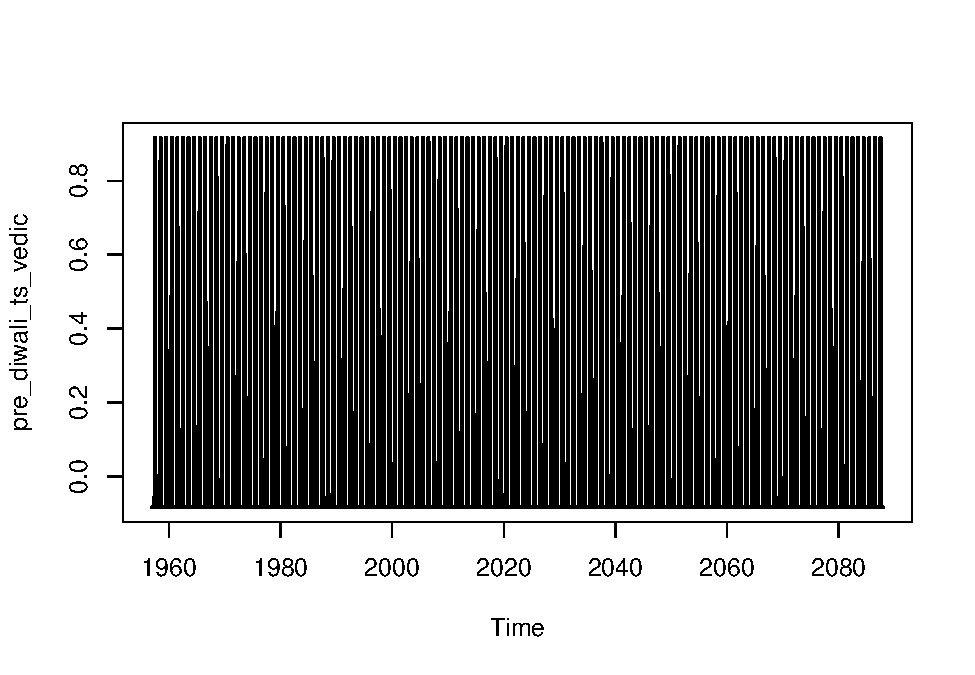
\includegraphics{regressors_of_diwali_seasonality_for_industrial_production_files/figure-latex/unnamed-chunk-6-1.pdf}

\begin{Shaded}
\begin{Highlighting}[]
\FunctionTok{ts.plot}\NormalTok{(post\_diwali\_ts\_vedic,}\AttributeTok{lwd =} \FunctionTok{c}\NormalTok{(}\DecValTok{2}\NormalTok{, }\DecValTok{1}\NormalTok{))}
\end{Highlighting}
\end{Shaded}

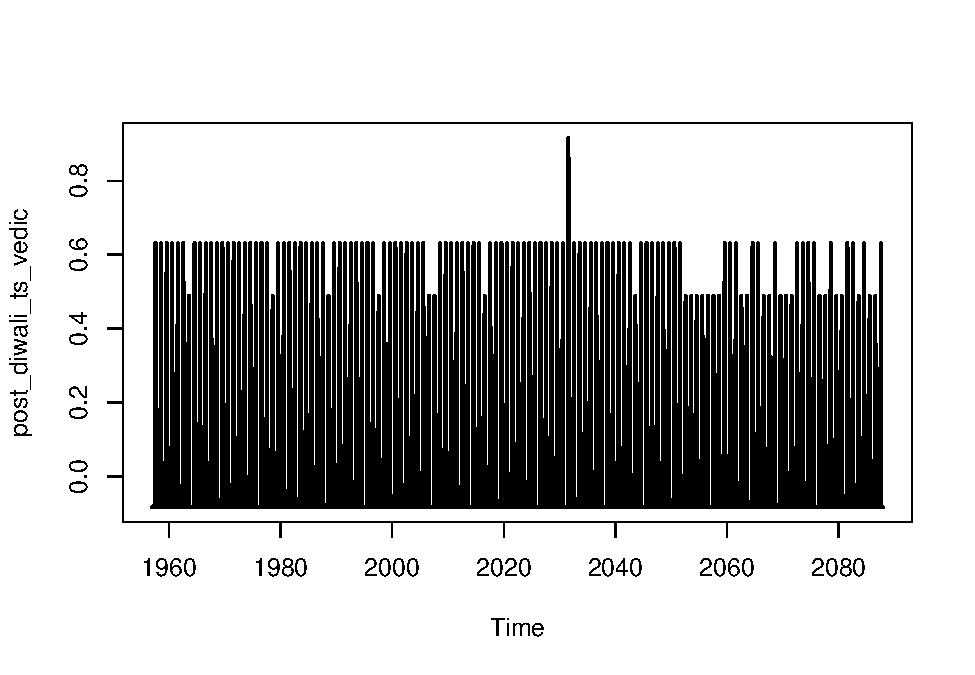
\includegraphics{regressors_of_diwali_seasonality_for_industrial_production_files/figure-latex/unnamed-chunk-6-2.pdf}

\hypertarget{generate-time-series-with-gregorian-calendar-system-for-diwali}{%
\paragraph{Generate time-series with Gregorian calendar system for
Diwali}\label{generate-time-series-with-gregorian-calendar-system-for-diwali}}

\begin{Shaded}
\begin{Highlighting}[]
\NormalTok{pre\_diwali\_ts}\OtherTok{\textless{}{-}} \FunctionTok{genhol}\NormalTok{(seasonal}\SpecialCharTok{::}\NormalTok{diwali, }\AttributeTok{start =} \SpecialCharTok{{-}}\DecValTok{6}\NormalTok{, }\AttributeTok{end =} \SpecialCharTok{{-}}\DecValTok{1}\NormalTok{, }\AttributeTok{center =} \StringTok{"mean"}\NormalTok{)}
\NormalTok{post\_diwali\_ts}\OtherTok{\textless{}{-}} \FunctionTok{genhol}\NormalTok{(seasonal}\SpecialCharTok{::}\NormalTok{diwali, }\AttributeTok{start =} \DecValTok{0}\NormalTok{, }\AttributeTok{end =} \DecValTok{6}\NormalTok{, }\AttributeTok{center =} \StringTok{"mean"}\NormalTok{)}
\FunctionTok{ts.plot}\NormalTok{(pre\_diwali\_ts,}\AttributeTok{lwd =} \FunctionTok{c}\NormalTok{(}\DecValTok{2}\NormalTok{, }\DecValTok{1}\NormalTok{))}
\end{Highlighting}
\end{Shaded}

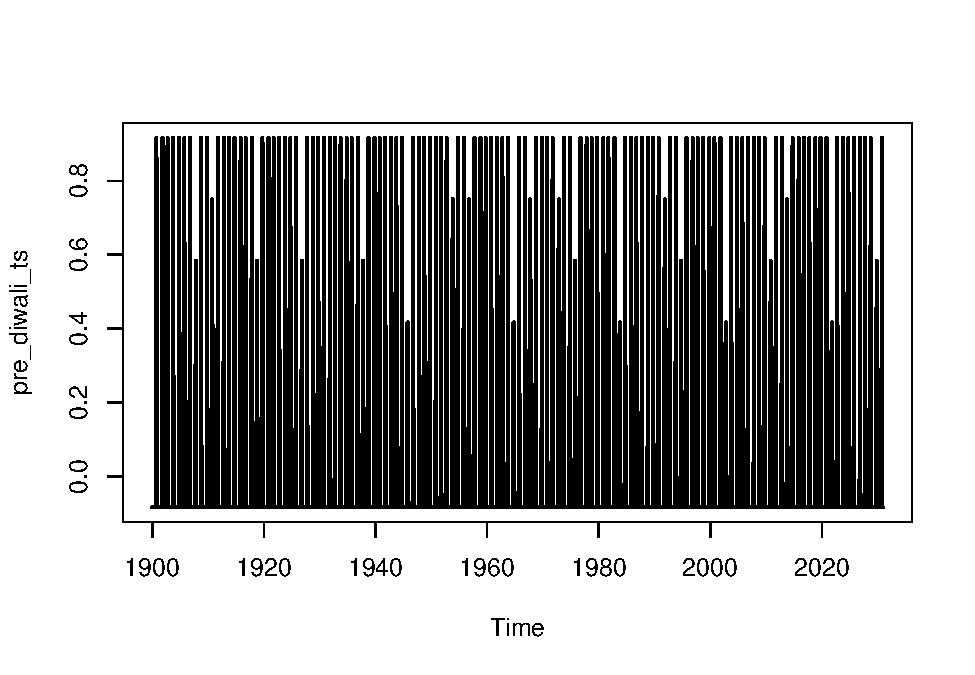
\includegraphics{regressors_of_diwali_seasonality_for_industrial_production_files/figure-latex/unnamed-chunk-7-1.pdf}

\begin{Shaded}
\begin{Highlighting}[]
\FunctionTok{ts.plot}\NormalTok{(post\_diwali\_ts,}\AttributeTok{lwd =} \FunctionTok{c}\NormalTok{(}\DecValTok{2}\NormalTok{, }\DecValTok{1}\NormalTok{))}
\end{Highlighting}
\end{Shaded}

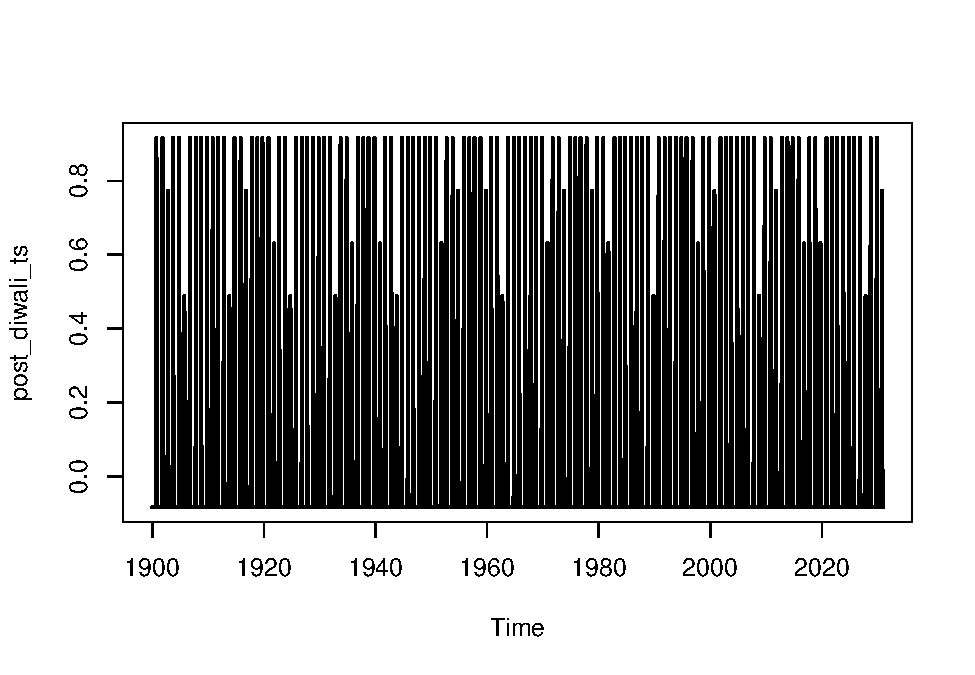
\includegraphics{regressors_of_diwali_seasonality_for_industrial_production_files/figure-latex/unnamed-chunk-7-2.pdf}

\hypertarget{including-user-defined-regressors}{%
\subsubsection{Including user defined
regressors}\label{including-user-defined-regressors}}

\hypertarget{converting-india-industrial-output-time-series-object-to-vedic-calendar-system}{%
\subsubsection{Converting India Industrial Output time-series object to
Vedic Calendar
system}\label{converting-india-industrial-output-time-series-object-to-vedic-calendar-system}}

Converting `seasonal::iip` ts object to Vedic calendar based time-series
object to model seasonality\\

\begin{Shaded}
\begin{Highlighting}[]
\NormalTok{iip\_data }\OtherTok{\textless{}{-}} \FunctionTok{data.frame}\NormalTok{(}\AttributeTok{Y=}\FunctionTok{as.matrix}\NormalTok{(seasonal}\SpecialCharTok{::}\NormalTok{iip), }\AttributeTok{date=}\FunctionTok{as.Date}\NormalTok{(zoo}\SpecialCharTok{::}\FunctionTok{as.yearmon}\NormalTok{(}\FunctionTok{time}\NormalTok{(seasonal}\SpecialCharTok{::}\NormalTok{iip))))}
\NormalTok{date}\OtherTok{\textless{}{-}}\NormalTok{ iip\_data}\SpecialCharTok{$}\NormalTok{date}
\NormalTok{date }\OtherTok{\textless{}{-}} \FunctionTok{as.POSIXct.Date}\NormalTok{(date)}
\NormalTok{julianday\_iip }\OtherTok{\textless{}{-}}\NormalTok{ insol}\SpecialCharTok{::}\FunctionTok{JD}\NormalTok{(date)}
\NormalTok{place }\OtherTok{\textless{}{-}} \FunctionTok{c}\NormalTok{(}\FloatTok{15.34}\NormalTok{, }\FloatTok{75.13}\NormalTok{, }\SpecialCharTok{+}\FloatTok{5.5}\NormalTok{) }\CommentTok{\#Latitude, Longitude and timezone of the location}
\NormalTok{iip\_vedic\_calendar }\OtherTok{=} \FunctionTok{c}\NormalTok{()}
\ControlFlowTok{for}\NormalTok{ (i }\ControlFlowTok{in} \DecValTok{1}\SpecialCharTok{:}\FunctionTok{length}\NormalTok{(julianday\_iip)) }
\NormalTok{\{}
\NormalTok{iip\_vedic\_calendar }\OtherTok{=} \FunctionTok{c}\NormalTok{(iip\_vedic\_calendar, }\FunctionTok{get\_vedic\_date}\NormalTok{(julianday\_iip[i], place))}
\NormalTok{\}}
\NormalTok{iip\_data}\SpecialCharTok{$}\NormalTok{date }\OtherTok{\textless{}{-}}\NormalTok{ iip\_vedic\_calendar}
\NormalTok{iip\_vedic\_data\_ts }\OtherTok{\textless{}{-}} \FunctionTok{ts}\NormalTok{(iip\_data}\SpecialCharTok{$}\NormalTok{Y,}\AttributeTok{start=}\FunctionTok{c}\NormalTok{(}\DecValTok{2061}\NormalTok{,}\DecValTok{2}\NormalTok{))}
\NormalTok{iip\_vedic\_data\_ts}
\end{Highlighting}
\end{Shaded}

\begin{verbatim}
## Time Series:
## Start = 2062 
## End = 2177 
## Frequency = 1 
##   [1]  99.0838 103.0900 103.9666 102.4425 104.1004 104.4108 107.3272 104.6366
##   [9] 116.8191 118.4664 112.4255 126.7159 108.8396 114.8274 114.2126 117.6044
##  [17] 114.2655 118.1773 117.6792 125.5368 132.7696 134.8564 127.8147 144.8739
##  [25] 128.2021 136.8587 136.7408 136.6459 134.5998 133.9824 140.7213 137.9242
##  [33] 150.7315 152.5200 149.3196 161.8845 142.3296 146.7452 148.3757 144.2976
##  [41] 141.8657 148.5866 146.1718 139.6522 148.2840 144.3709 138.5057 153.5340
##  [49] 139.5905 144.2723 145.7417 146.7192 149.4225 151.0090 149.6481 148.4985
##  [57] 162.3779 163.6191 157.5185 176.4743 157.8465 156.5436 156.5543 161.3000
##  [65] 156.1000 160.3000 166.6000 158.0000 175.6000 175.9000 168.0000 193.1000
##  [73] 166.2000 166.2000 171.4000 167.2000 161.4000 164.3000 158.3000 167.5000
##  [81] 180.3000 177.6000 175.2000 187.6000 164.1000 170.3000 168.0000 167.1000
##  [89] 164.7000 163.1000 171.6000 165.8000 179.3000 182.0000 176.2000 194.2000
##  [97] 166.5000 166.0000 164.9000 171.4000 165.4000 167.5000 169.6000 163.6000
## [105] 179.5000 184.0000 172.7000 193.3000 172.7000 175.3000 172.0000 173.0000
## [113] 166.2000 172.2000 162.5000 169.8000
\end{verbatim}

The \texttt{seasonal} package allows to add user-defined regressors to
remove seasonality from a time-series. Here \texttt{pre\_diwali\_ts} and
\texttt{post\_diwali\_ts} are added in the main seasonal adjustment.
\texttt{X-13ARIMA-SEATS} is used to adjust for the festival seasonal
component.

\begin{Shaded}
\begin{Highlighting}[]
\NormalTok{m1 }\OtherTok{\textless{}{-}} \FunctionTok{seas}\NormalTok{(industrial\_prod, }\AttributeTok{xreg =} \FunctionTok{cbind}\NormalTok{(pre\_diwali\_ts, post\_diwali\_ts), }\AttributeTok{regression.usertype =} \StringTok{"holiday"}\NormalTok{, }\AttributeTok{x11 =} \FunctionTok{list}\NormalTok{())}
\end{Highlighting}
\end{Shaded}

\texttt{xreg} adds the user-defined regressors and \texttt{x11} is
chosen as the decomposition effect.

\begin{Shaded}
\begin{Highlighting}[]
\FunctionTok{summary}\NormalTok{(m1)}
\end{Highlighting}
\end{Shaded}

\begin{verbatim}
## 
## Call:
## seas(x = industrial_prod, xreg = cbind(pre_diwali_ts, post_diwali_ts), 
##     regression.usertype = "holiday", x11 = list())
## 
## Coefficients:
##                     Estimate Std. Error z value Pr(>|z|)    
## xreg1             -0.0034498  0.0091813  -0.376  0.70711    
## xreg2             -0.0383834  0.0081358  -4.718 2.38e-06 ***
## Weekday            0.0012087  0.0004275   2.827  0.00469 ** 
## Constant          -0.0014297  0.0003227  -4.431 9.39e-06 ***
## LS2008.Nov        -0.0738919  0.0160213  -4.612 3.99e-06 ***
## MA-Nonseasonal-01  0.4328295  0.0785625   5.509 3.60e-08 ***
## MA-Seasonal-12     0.9995753  0.0785461  12.726  < 2e-16 ***
## ---
## Signif. codes:  0 '***' 0.001 '**' 0.01 '*' 0.05 '.' 0.1 ' ' 1
## 
## X11 adj.  ARIMA: (0 1 1)(0 1 1)  Obs.: 116  Transform: log
## AICc: 543.2, BIC: 562.7  QS (no seasonality in final):    0  
## Box-Ljung (no autocorr.): 31.53   Shapiro (normality): 0.9894
\end{verbatim}

The seasonal co-efficient shows minor decline during pre and post Diwali
season across the time-series. In the below unadjusted v adjusted
seasonal plot it can be observed that seasonal adjustment based on
Diwali season removes distortion from the time-series.

\begin{Shaded}
\begin{Highlighting}[]
\FunctionTok{plot}\NormalTok{(m1)}
\FunctionTok{lines}\NormalTok{(iip\_vedic\_data\_ts, }\AttributeTok{col=}\StringTok{"red"}\NormalTok{)}
\end{Highlighting}
\end{Shaded}

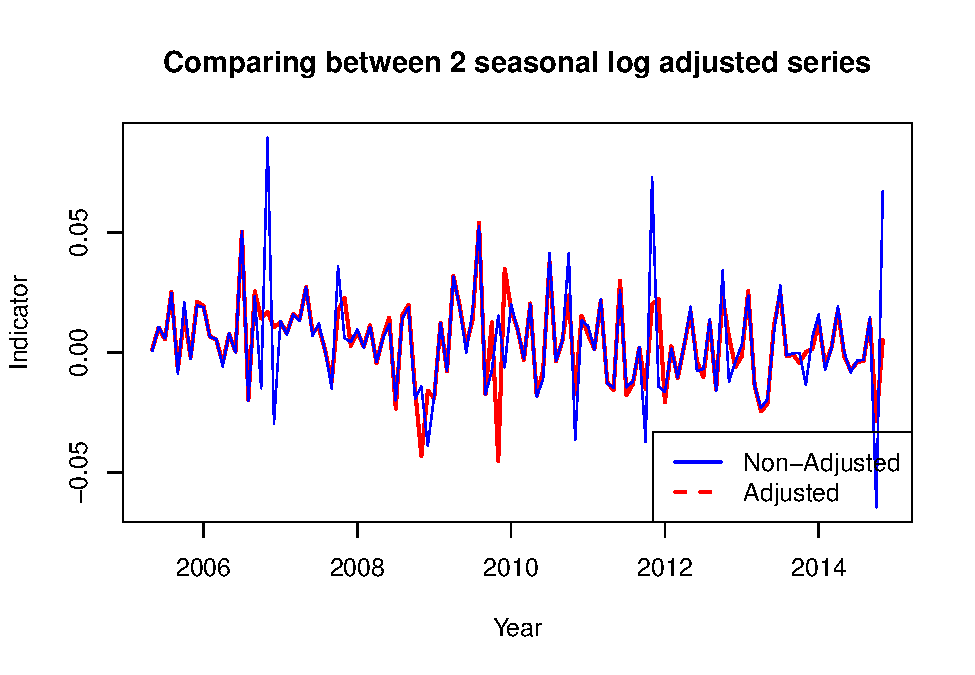
\includegraphics{regressors_of_diwali_seasonality_for_industrial_production_files/figure-latex/unnamed-chunk-11-1.pdf}

\hypertarget{comparing-the-series}{%
\subsubsection{Comparing the series}\label{comparing-the-series}}

\begin{Shaded}
\begin{Highlighting}[]
\NormalTok{m2 }\OtherTok{\textless{}{-}} \FunctionTok{seas}\NormalTok{(}\AttributeTok{x =}\NormalTok{ iip, }\AttributeTok{x11 =} \FunctionTok{list}\NormalTok{(), }\AttributeTok{regression.variables =} \FunctionTok{c}\NormalTok{(}\StringTok{"td1coef"}\NormalTok{, }\StringTok{"ls2008.Nov"}\NormalTok{), }
           \AttributeTok{arima.model =} \StringTok{"(0 1 1)(0 1 1)"}\NormalTok{, }\AttributeTok{regression.aictest =} \ConstantTok{NULL}\NormalTok{, }\AttributeTok{outlier =} \ConstantTok{NULL}\NormalTok{, }
           \AttributeTok{transform.function =} \StringTok{"log"}\NormalTok{)}
\FunctionTok{ts.plot}\NormalTok{(}\FunctionTok{diff}\NormalTok{(}\FunctionTok{log}\NormalTok{(}\FunctionTok{cbind}\NormalTok{(}\FunctionTok{final}\NormalTok{(m1), }\FunctionTok{final}\NormalTok{(m2)))), }\AttributeTok{col =} \FunctionTok{c}\NormalTok{(}\StringTok{"red"}\NormalTok{, }\StringTok{"blue"}\NormalTok{), }
        \AttributeTok{lwd =} \FunctionTok{c}\NormalTok{(}\DecValTok{2}\NormalTok{, }\DecValTok{1}\NormalTok{))}
\end{Highlighting}
\end{Shaded}

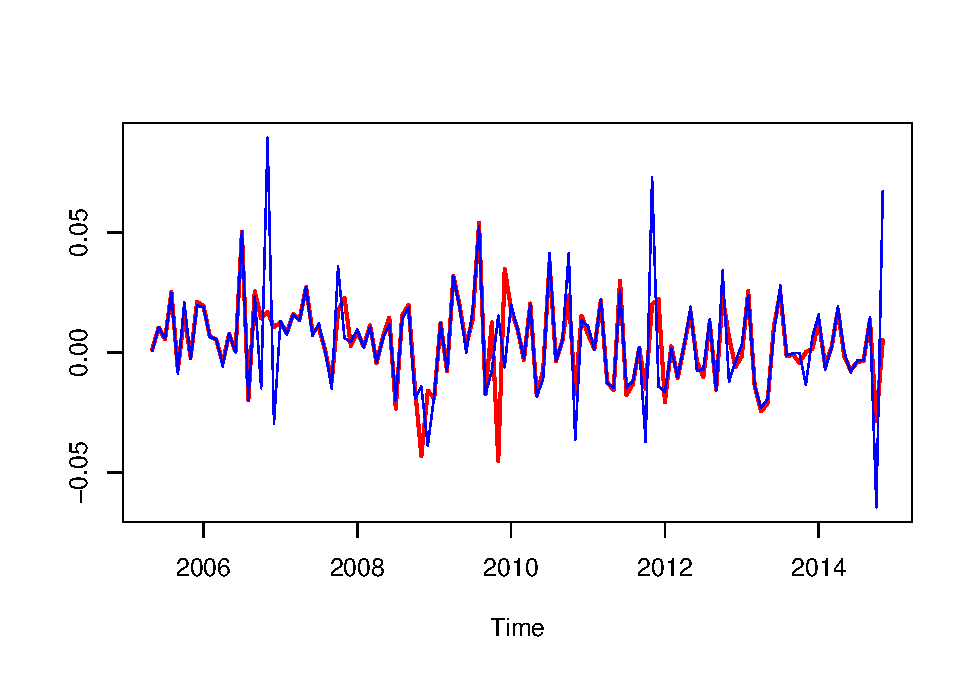
\includegraphics{regressors_of_diwali_seasonality_for_industrial_production_files/figure-latex/unnamed-chunk-12-1.pdf}

In the above chart, non-adjusted(blue) vs adjusted(red) seasonal plot
clearly shows the amount of distortion present in the series.

The below chart also indicated a level of distortion present for
industrial output due to Diwali festival.

\begin{Shaded}
\begin{Highlighting}[]
\FunctionTok{ts.plot}\NormalTok{(}\FunctionTok{final}\NormalTok{(m1), }\FunctionTok{final}\NormalTok{(m2), }\AttributeTok{col =} \FunctionTok{c}\NormalTok{(}\StringTok{"red"}\NormalTok{, }\StringTok{"blue"}\NormalTok{), }\AttributeTok{lwd =} \FunctionTok{c}\NormalTok{(}\DecValTok{2}\NormalTok{, }\DecValTok{1}\NormalTok{))}
\end{Highlighting}
\end{Shaded}

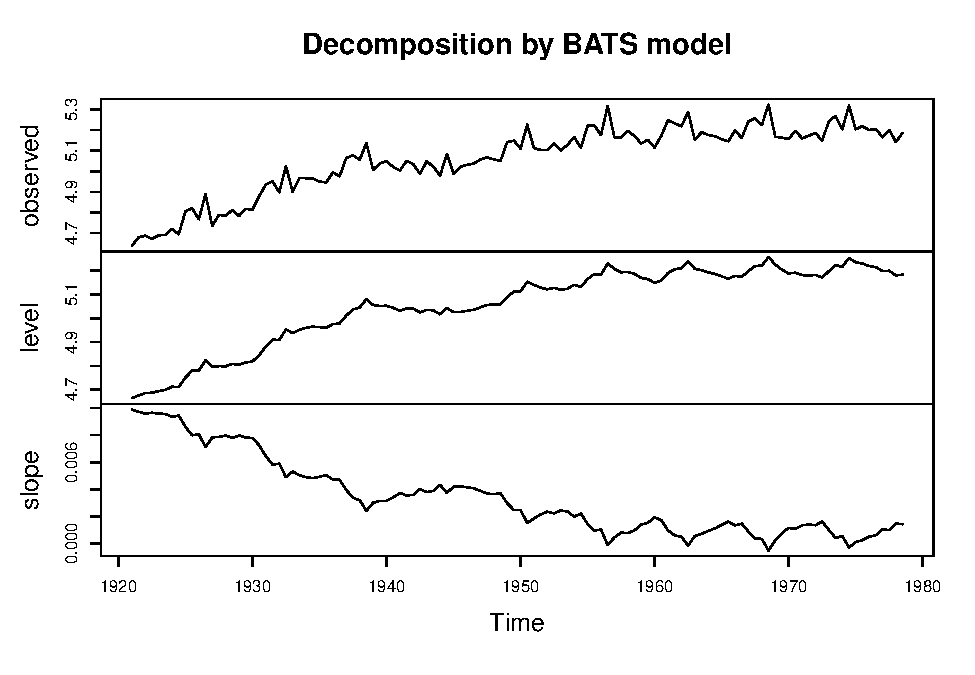
\includegraphics{regressors_of_diwali_seasonality_for_industrial_production_files/figure-latex/unnamed-chunk-13-1.pdf}

\hypertarget{multi-seasonality-decomposition-for-india-industrial-output}{%
\subsection{Multi-seasonality decomposition for India industrial
output}\label{multi-seasonality-decomposition-for-india-industrial-output}}

(\textbf{forecast?}) library was used to identify multiple seasonality
present in the data-set and understand the difference between them.

\hypertarget{seasonality-decomposition-for-industrial-output-for-gregorian-calendar}{%
\subsubsection{Seasonality decomposition for Industrial Output for
Gregorian
Calendar}\label{seasonality-decomposition-for-industrial-output-for-gregorian-calendar}}

The start of the series is from year 2000 according to Gregoriann
calendar system

\begin{Shaded}
\begin{Highlighting}[]
\NormalTok{iip\_tbats }\OtherTok{\textless{}{-}}\NormalTok{ forecast}\SpecialCharTok{::}\FunctionTok{msts}\NormalTok{(industrial\_prod, }\AttributeTok{start=}\DecValTok{2000}\NormalTok{, }\AttributeTok{seasonal.periods =} \FunctionTok{c}\NormalTok{(}\DecValTok{1}\NormalTok{))}
\NormalTok{fit }\OtherTok{\textless{}{-}}\NormalTok{ forecast}\SpecialCharTok{::}\FunctionTok{tbats}\NormalTok{(iip\_tbats)}
\FunctionTok{plot}\NormalTok{(fit)}
\end{Highlighting}
\end{Shaded}

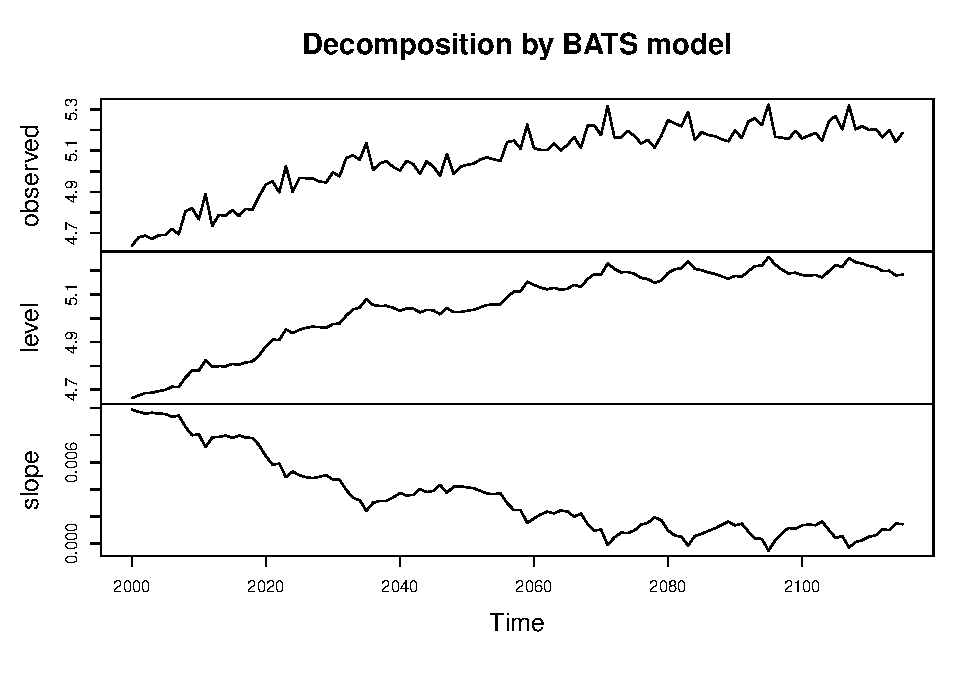
\includegraphics{regressors_of_diwali_seasonality_for_industrial_production_files/figure-latex/unnamed-chunk-14-1.pdf}

\hypertarget{seasonality-decomposition-for-industrial-output-for-vedic-calendar}{%
\subsubsection{Seasonality decomposition for Industrial Output for Vedic
Calendar}\label{seasonality-decomposition-for-industrial-output-for-vedic-calendar}}

The start of the series is 1921, according to Vedic calendar system
which is equivalent to 2000

\begin{Shaded}
\begin{Highlighting}[]
\NormalTok{iip\_tbats\_vedic }\OtherTok{\textless{}{-}}\NormalTok{ forecast}\SpecialCharTok{::}\FunctionTok{msts}\NormalTok{(iip\_vedic\_data\_ts, }\AttributeTok{start=}\DecValTok{1921}\NormalTok{, }\AttributeTok{seasonal.periods =} \FunctionTok{c}\NormalTok{(}\DecValTok{2}\NormalTok{))}
\NormalTok{fit\_vedic }\OtherTok{\textless{}{-}}\NormalTok{ forecast}\SpecialCharTok{::}\FunctionTok{tbats}\NormalTok{(iip\_tbats\_vedic)}
\FunctionTok{plot}\NormalTok{(fit\_vedic)}
\end{Highlighting}
\end{Shaded}

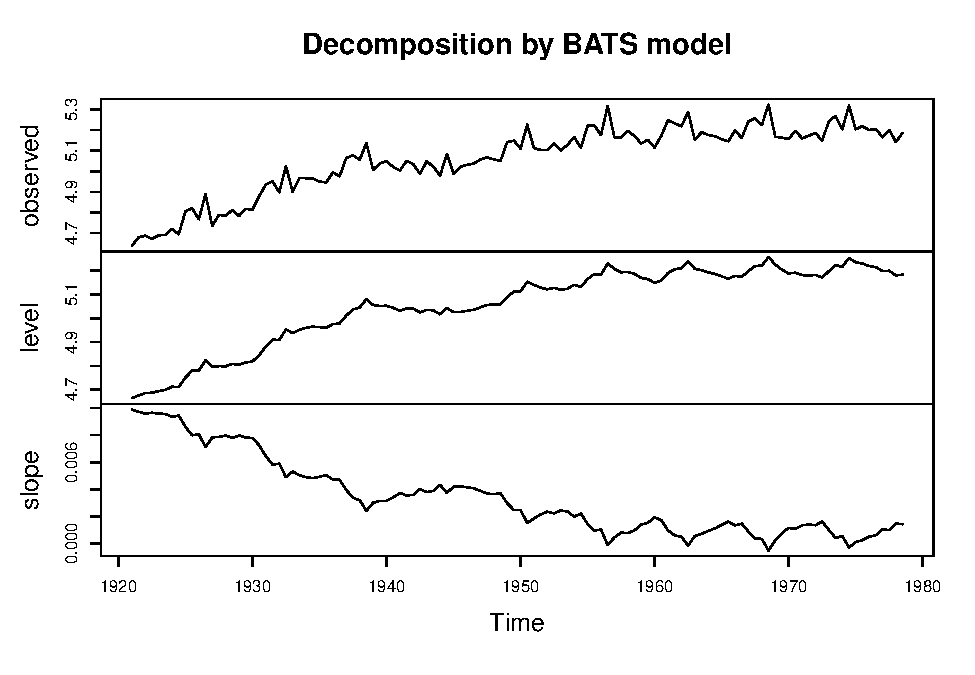
\includegraphics{regressors_of_diwali_seasonality_for_industrial_production_files/figure-latex/unnamed-chunk-15-1.pdf}

\hypertarget{refs}{}
\begin{CSLReferences}{1}{0}
\leavevmode\vadjust pre{\hypertarget{ref-seasonal}{}}%
Sax, Christoph, and Dirk Eddelbuettel. 2018. {``Seasonal Adjustment by
{\textbraceleft}x-13ARIMA-SEATS{\textbraceright} in
{\textbraceleft}r{\textbraceright}''} 87.
\url{https://doi.org/10.18637/jss.v087.i11}.

\end{CSLReferences}

\end{document}
